\documentclass[12pt]{article}
\usepackage[english]{babel}
\usepackage{natbib}
\usepackage{url}
\usepackage[utf8]{inputenc}
\usepackage{amsmath}
\usepackage{amssymb}
\usepackage{graphicx}
\usepackage{parskip}
\usepackage{fancyhdr}
\usepackage{vmargin}
\usepackage{booktabs}
\usepackage[table,xcdraw]{xcolor}
\usepackage{tabularx}
\usepackage{caption} 
\usepackage{float}
\usepackage{longtable}
\usepackage{array}
\usepackage{caption}
\usepackage{subcaption}

\setmarginsrb{3 cm}{1 cm}{3 cm}{1 cm}{1 cm}{1.5 cm}{1 cm}{1.5 cm}

\newcolumntype{L}[1]{>{\raggedright\let\newline\\\arraybackslash\hspace{0pt}}m{#1}}
\newcolumntype{C}[1]{>{\centering\let\newline\\\arraybackslash\hspace{0pt}}m{#1}}
\newcolumntype{R}[1]{>{\raggedleft\let\newline\\\arraybackslash\hspace{0pt}}m{#1}}

\usepackage{natbib}

\title{Assignment \#3 - Population Testing}
\date{\today}

\makeatletter
\let\thetitle\@title
\let\thesubtitle\@subtitle
\let\theauthor\@author
\let\thedate\@date
\makeatother

\pagestyle{plain}

\captionsetup[table]{skip=5pt}


\begin{document}

%%%%%%%%%%%%%%%%%%%%%%%%%%%%%%%%%%%%%%%%%%%%%%%%%%%%%%%%%%%%%%%%%%%%%%%%%%%%%%%%%%%%%%%%%

\begin{titlepage}
	\centering
    \textsc{\LARGE University of Coimbra}\\[1.0 cm]
	\textsc{\large Doctoral Program in Information Science and Technology}\\[0.5 cm]
    \textsc{\large Statistics}\\[5 cm]
	\rule{\linewidth}{0.2 mm} \\[0.4 cm]
	{ \LARGE \bfseries \thetitle}\\ [0.2 cm]
    \rule{\linewidth}{0.2 mm} \\[3 cm]
    
    \textsc{Joaquim Pedro Bento Gonçalves Pratas Leitão - 2011150072}\\[5 cm]
	
	{\large \thedate}\\[2 cm]
 
	\vfill
	
\end{titlepage}

%%%%%%%%%%%%%%%%%%%%%%%%%%%%%%%%%%%%%%%%%%%%%%%%%%%%%%%%%%%%%%%%%%%%%%%%%%%%%%%%%%%%%%%%%

\section{Introduction}
\label{introduction}

The current document is framed in the scope of the third assignment of the Statistics course, taught for the Doctoral Program in Information Science and Technology at the University of Coimbra, during the academic year of 2016/2017.

The current assignment focus on parametric and non-parametric significance tests with respect to the average of a given population of which a sample was observed and collected.

The data collected for this assignment through a survey of fast-food consumption habits in England was used in this study, and the opinions of $344$ consumers who reported buying fast food regularly were recorded. The supplied dataset contains the following variables:

\begin{itemize}
	\item Average number of weekly fast-food purchases in the last month.
	
	\item Age of the reporting person, divided in five classes: \textbf{1} for people with ages between 15 and 17, \textbf{2} for 18-24, \textbf{3} for 25-35, \textbf{4} for 36-54 and \textbf{5} for 55-70.

	\item Genre of the reporting person.
	
	\item Socio-economic level of the reporting person, divided in three classes: \textbf{1} for low, \textbf{2} for medium and \textbf{3} for high.
	
	\item Educational qualifications of the reporting person, divided in four classes: \textbf{1} for high school level, \textbf{2} for technical course, \textbf{3} for B.Sc degree and \textbf{4} for MSc or PhD.
\end{itemize}

As already mentioned, the main focus and goal of the current assignment was on the application of adequate parametric and non-parametric significance tests to the collected and observed samples, in order to withdraw conclusions with respect to the entire population under study.

The main variable under analysis is the average number of weekly fast-food purchases, and the three tests proposed for the current assignment relate this variable with some of the remaining collected variables: In the first two tests fast-food purchases are related with the genre of the inquired people and in the final test an analysis of fast-food purchases by age is performed.

As required, all tests were performed with a significance level of $0.05$. In addition, all tests documented in this report were performed using the \emph{R}\footnote{\url{https://www.r-project.org/}} software environment.

In the remainder of this document the tests proposed in the current assignment will be covered: In section \ref{genre_tests} the first two tests are presented and discussed, while section \ref{age_tests} is reserved for the third test.

\section{Fast-Food Purchases by Genre}
\label{genre_tests}

In the current section the two proposed tests to relate fast-food purchases with the survey respondents' genre are covered.

\subsection{Purchases by Women}

As a starting point it was intended to analyse the average fast-food purchases made by women, in order to determine whether or not this average value (in the previous month) was significantly higher than a given value, 2.5 in our scenario.

Taking into account that only one variable was being analysed at this point (corresponding to a subset of the collected sample) we are faced with a test for the average of a population, which may or may not be parametric. Therefore, a \emph{Student's T-Test} (T-Test) appears as the most promising test, provided its assumptions can be met.

Since the T-Test assumes the random variable in question follows a normal distribution, the initial step in this problem will be determining whether or not the variable of interest (in this case, the average fast-food purchases made in the last month) follows a normal distribution.

To this end, a \emph{Shapiro-Wilk} test for normality in the variable of interest was performed. A \emph{p-value} of $7.191026e^{-12}$ was registered in this test. As this \emph{p-value} is considerably smaller than the required significance level, the test's null hypothesis (stating that the variable under analysis follows a normal distribution) is rejected, at the significance level of $0.05$.

These results are further supported by the histogram of the average fast-food purchases by women, presented in figure \ref{histogram_women_purchases}.

\begin{figure}[H]
	\centering
	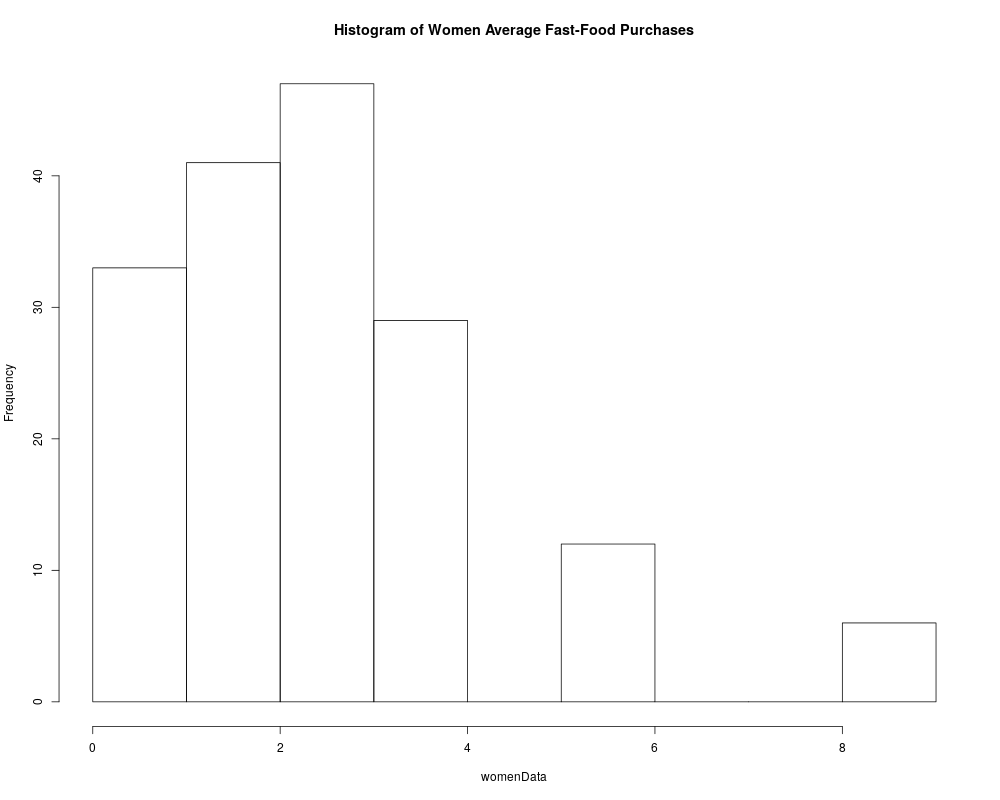
\includegraphics[scale=0.28]{images/Histogram_WomenData.png}
	\caption{Histogram of fast-food purchases by women.}
	\label{histogram_women_purchases}
\end{figure}

A practical result of the application of the \emph{Shapiro-Wilk} test for the fast-food purchases by women implies that this variable cannot be accepted to follow a normal distribution.

Even though normality cannot be assured for our study variable, the T-Test  can still be applied to this variable, provided its number of observations is higher than $30$. In this case we obtain an approximate \emph{p-value} for the test. Considering that a total of $168$ women answered the survey, the T-Test can still be applied to the fast-food purchases made by women (as $168 > 30$).

As a result, the following hypothesis were considered in the T-Test:

$$ H0: \: m_{X} = 2.5 \: \: \: vs \: \: \: H1: m_{X} > 2.5$$

where \emph{X="Average number of weekly fast-food purchases made by women in the last month"}.

For this test a \emph{p-value} of $0.2779$ was registered. As this value is considerably higher than the required significance level ($0.05$) the null hypothesis is accepted, at this significance level. Such hypothesis states that the average number of weekly fast-food purchases made by women in the last month is 2.5.

Based on what was presented in this section and on the results of the performed hypothesis tests, the main conclusion to be withdrawn at this point is that it cannot be concluded that the average number of weekly fast-food purchases made by women in the last month is significantly higher than 2.5.

\subsection{Purchases by Women and Men}



\section{Fast-Food Purchases by Age}
\label{age_tests}


\end{document}